% \newcommand{\RomanNumeralCaps}[1]{\MakeUppercase{\romannum{#1}}.}
\chapter{General Project Context}
\label{chap: General Project Context}

\section*{Introduction}

This chapter provides a general overview of the host company, presenting its background, including its history and its current positioning in the market. It outlines the company’s areas of expertise, core mission, and vision. Additionally, the chapter introduces the project assigned during the internship, detailing its context, the problem it aims to address, and the proposed solution. It also presents the project brief, defining the functional and technical specifications of the project. Finally, this chapter highlights the project management methodology adopted  such as the Agile approach  and includes a Gantt chart to illustrate the planning and distribution of tasks over time.

\newpage

\phantomsection
\addcontentsline{toc}{section}{Presentation of Host Organization}
\section{Presentation of Host Organization}

 \subsection{History and Positioning}
 \begin{figure}[H] 
    \centering
    
\includegraphics[width=5cm]{Logos/Company_Logo.png}
    \caption{Company logo}
    %\label{fig:my_label} %Optional (If you want to reference the figure in later chapters)
\end{figure}

Founded in 2017 in Tétouan, Yafa Technologies is a Moroccan company located at 11, Avenue Zerktouni, Appart 12, Tétouan 93000. Since its creation, the company has steadily grown and established itself as a recognized player in the field of custom IT solutions and digital transformation services.

Through its commitment to innovation and quality, Yafa Technologies has built a strong reputation by responding effectively to the specific needs of both private companies and public institutions. Its strategic positioning focuses on developing tailored digital tools that help clients optimize their operations, improve productivity, and embrace technological change
    \subsection{Mission and Vision}

Yafa Technologies' mission is to provide reliable and secure IT solutions that support its clients in improving their operations and staying competitive. Its vision is to be a trusted partner in digital transformation, helping organizations make better decisions through the use of modern technologies and practical expertise..
    \subsection{ Areas of Expertise}

 Yafa Technologies offers a comprehensive suite of services, demonstrating its versatility and commitment to holistic client support. These include:
    \begin{itemize}
        \item \textbf{Custom Software Development:} Designing and implementing bespoke software applications tailored to specific business requirements.
        \item \textbf{Web and Mobile Application Development:} Creating intuitive and powerful applications to enhance user engagement and operational efficiency.
        \item \textbf{Data Analytics and Business Intelligence:} Providing solutions for data collection, processing, analysis, and visualization to derive actionable insights.
        \item \textbf{Cloud Computing Solutions:} Assisting organizations in migrating to and managing cloud infrastructure for enhanced scalability and flexibility.
        \item \textbf{IT Consulting and Professional Training:} Offering expert advice and customized training programs to build internal capacity and optimize IT strategies.
        \item \textbf{Cybersecurity Services:} Implementing robust security measures to protect digital assets and ensure data integrity.
    \end{itemize}









\subsection{Organizational Chart}

\begin{figure}[H] 
    \centering
    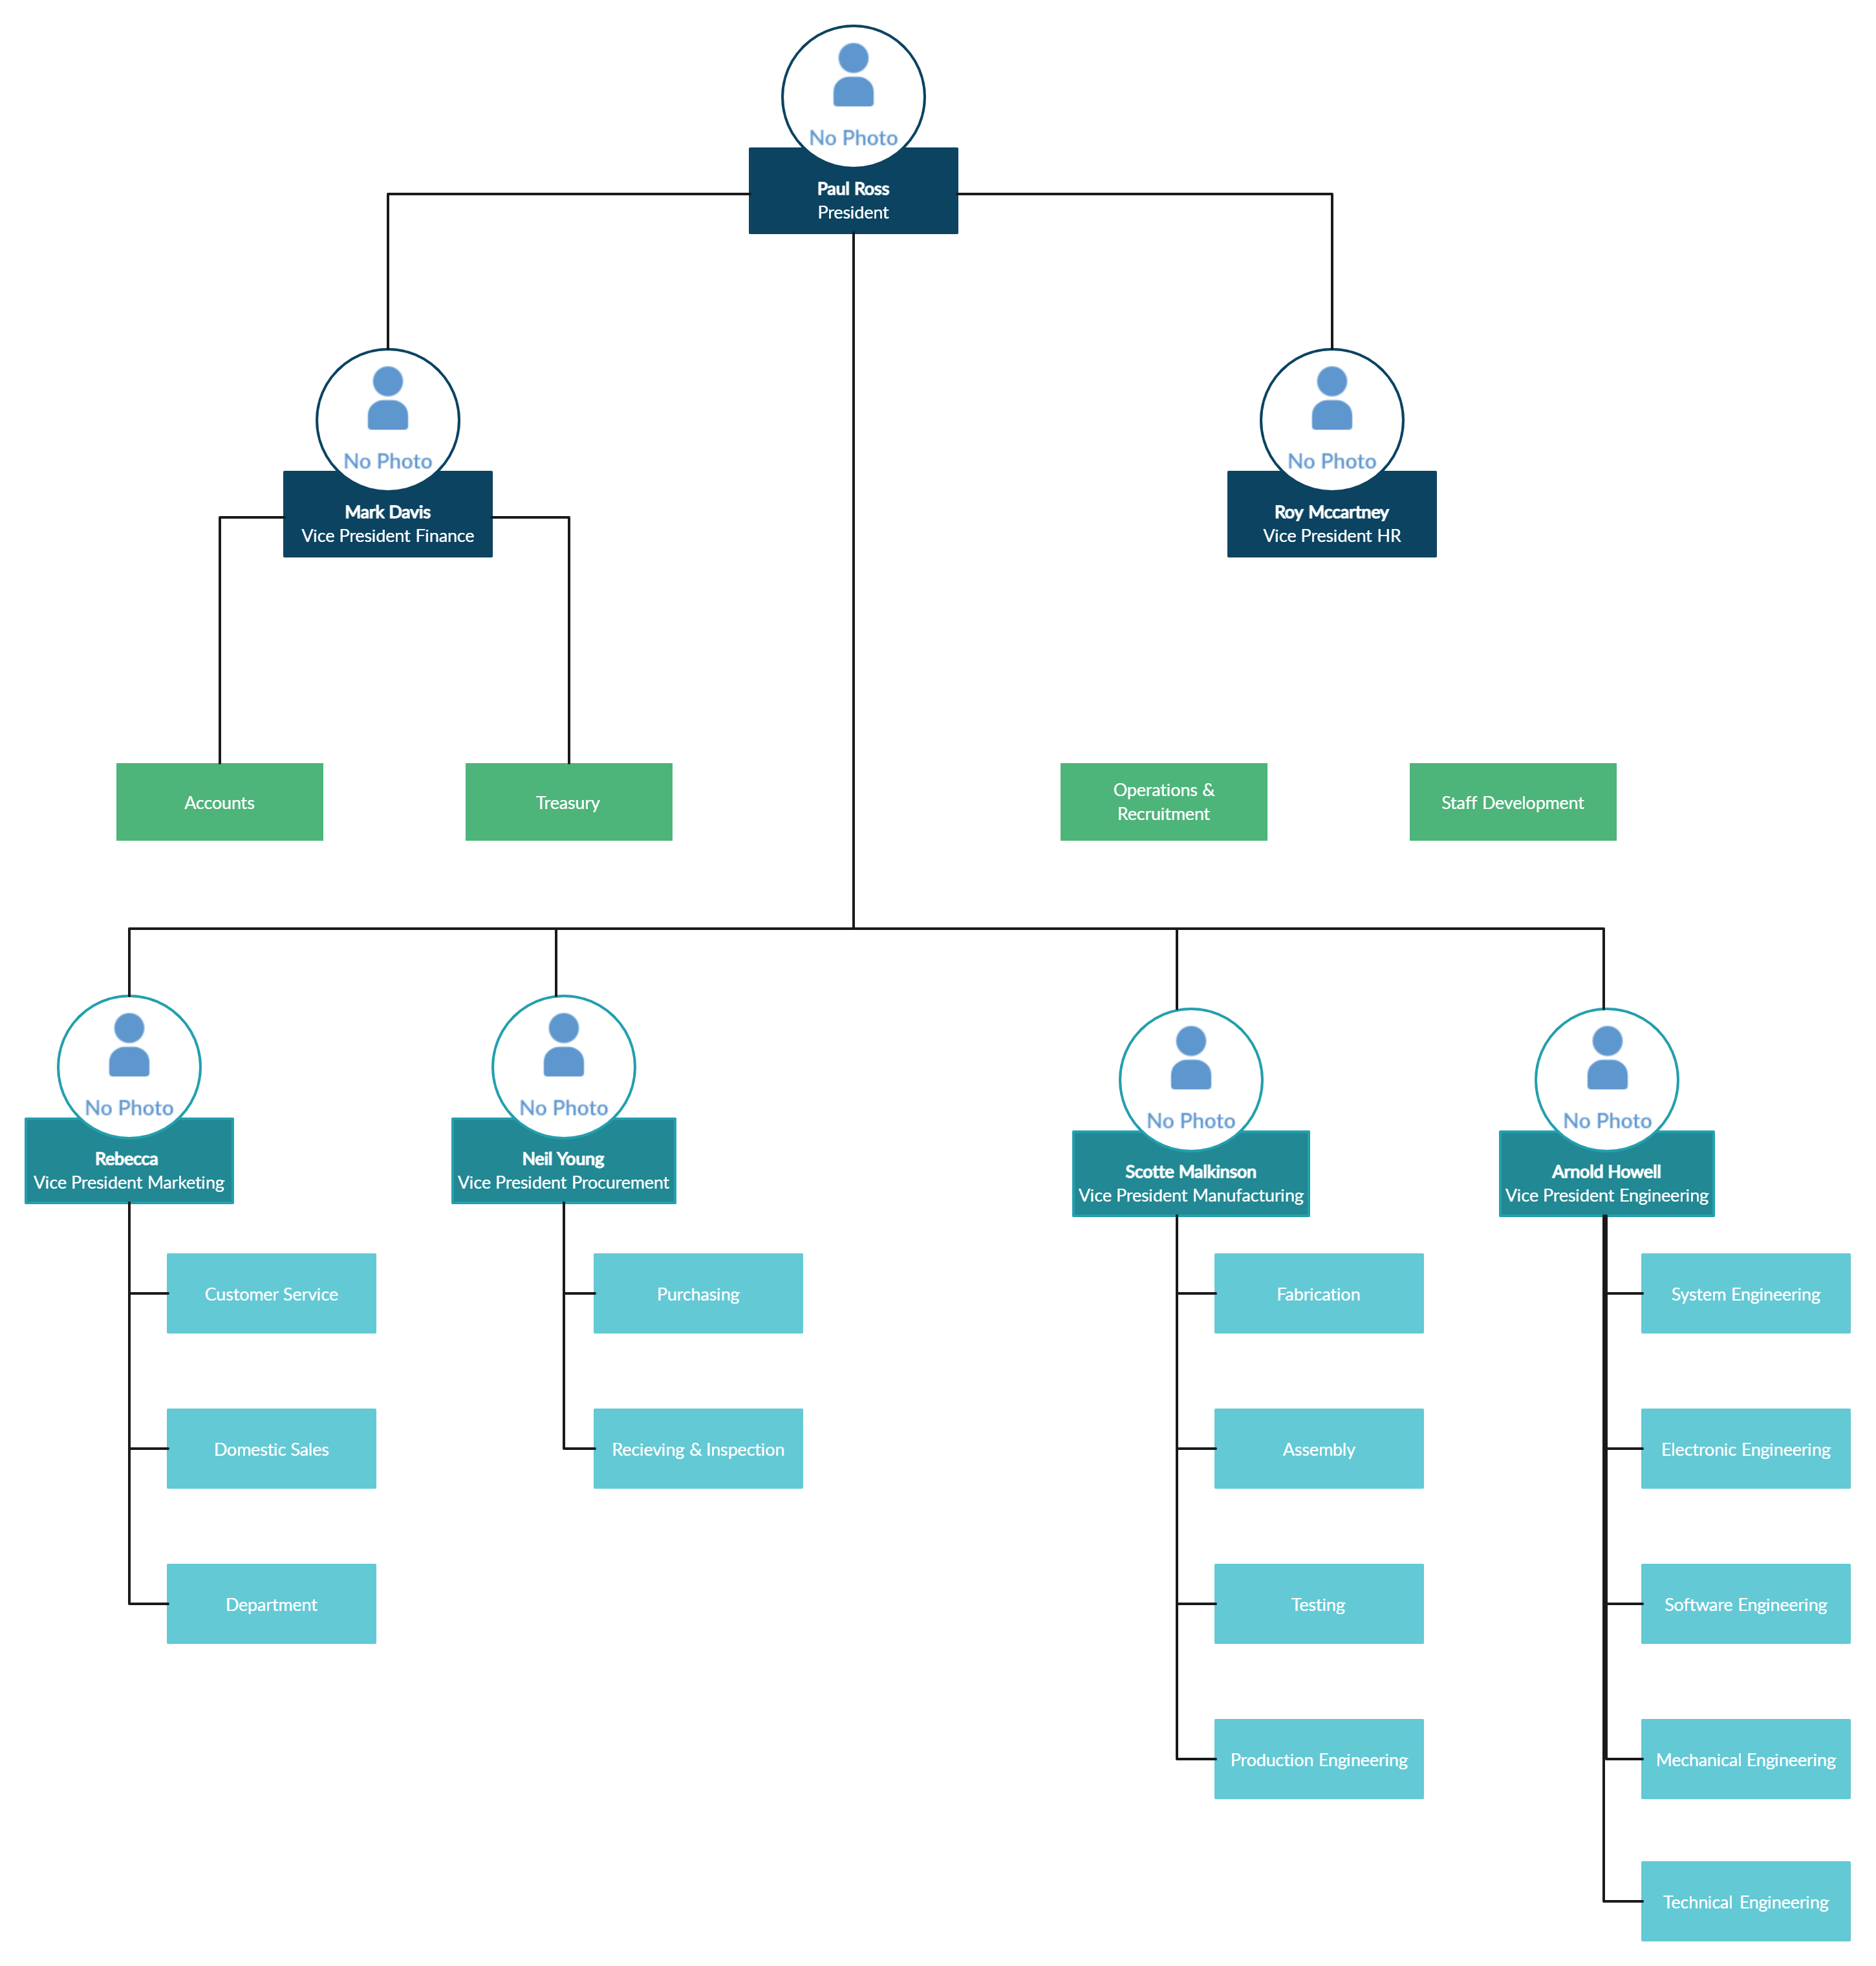
\includegraphics[width=1cm]{Figures/Organizational_Chart.png}
    \caption{Organizational Chart}
    %\label{fig:my_label} %Optional (If you want to reference the figure in later chapters)
\end{figure}


\section{Project Presentation}
\subsection{Topic Overview}


The main challenge of this project is to develop a comprehensive Federated Learning system that combines multiple key functions into a single platform. This system will enable the collaborative training of a time series model to predict the Water Quality Index (WQI) based on data collected from distributed sensors, all while maintaining data privacy by avoiding centralization of raw data. In addition to the model training process, the system will provide an administrative dashboard allowing authorized users to configure system parameters, monitor real-time performance metrics, and receive alerts in case of operational issues or anomalies. 

\subsection{Problematic}

 Traditional centralized approaches to water quality monitoring face several critical challenges:
    \begin{itemize}
        \item \textbf{Data Privacy:} Transmitting raw sensor data from multiple locations to a central server can raise significant privacy concerns, especially if data originates from private properties or regulated areas.
        \item \textbf{Communication Overhead:} Continuously streaming large volumes of sensor data can be bandwidth-intensive and costly, particularly in remote areas with limited connectivity.
        \item \textbf{Scalability:} Centralized systems can struggle to scale efficiently as the number of monitoring points increases, leading to bottlenecks in data processing and storage.
        \item \textbf{Latency:} Relying on cloud processing can introduce delays in detecting critical water quality issues, hindering rapid response.
        \item \textbf{Single Point of Failure:} A centralized server represents a single point of failure; if it goes down, the entire monitoring system can be compromised.
    \end{itemize}

% \subsection{Specifications document}

% TODO:

\subsection{Project Management}
\subsubsection{Agile Practices}
To allow flexibility and responsiveness during the process of creating the Federating Learning Project, Agile methods are incorporated into the process. The project is structured in phases with activities and milestones well-defined so that iterative improvements and continuous feedback incorporation can be accomplished. Each phase, from Formation and Study to Testing and Reporting, consists of an incremental development cycle, wherein the system progressively develops and fixes potential issues early in the process.

Agile methodology is observed through task dependency and concurrent processes in the project. For example, during the Environment Setup stage, certain of the preparatory tasks of Core Development can run in parallel to enable effective usage of resources. Ongoing teamwork and sprint planning allow for bottleneck detection and prioritization of the work to be done so that every development iteration contains a workable and testable component.

Moreover, Agile patterns such as frequent testing and validation are implemented, primarily during the Testing \& Reporting phase. Through continuous testing of the federated learning convergence of the system and security enhancement, feedback loops are established to enhance encryption processes and optimize model performance. Documentation refreshes at key points are also embraced by the project, with the PFE adapting in line with development and minimizing technical debt while optimizing knowledge transfer.

Using the Agile principles, the Federating Learning Project maintains responsiveness to changing needs, streamlines collaboration, and ensures delivery meets both the technical and business expectations.

\subsubsection{Internship Planning}
\begin{figure}[H]
    \centering
    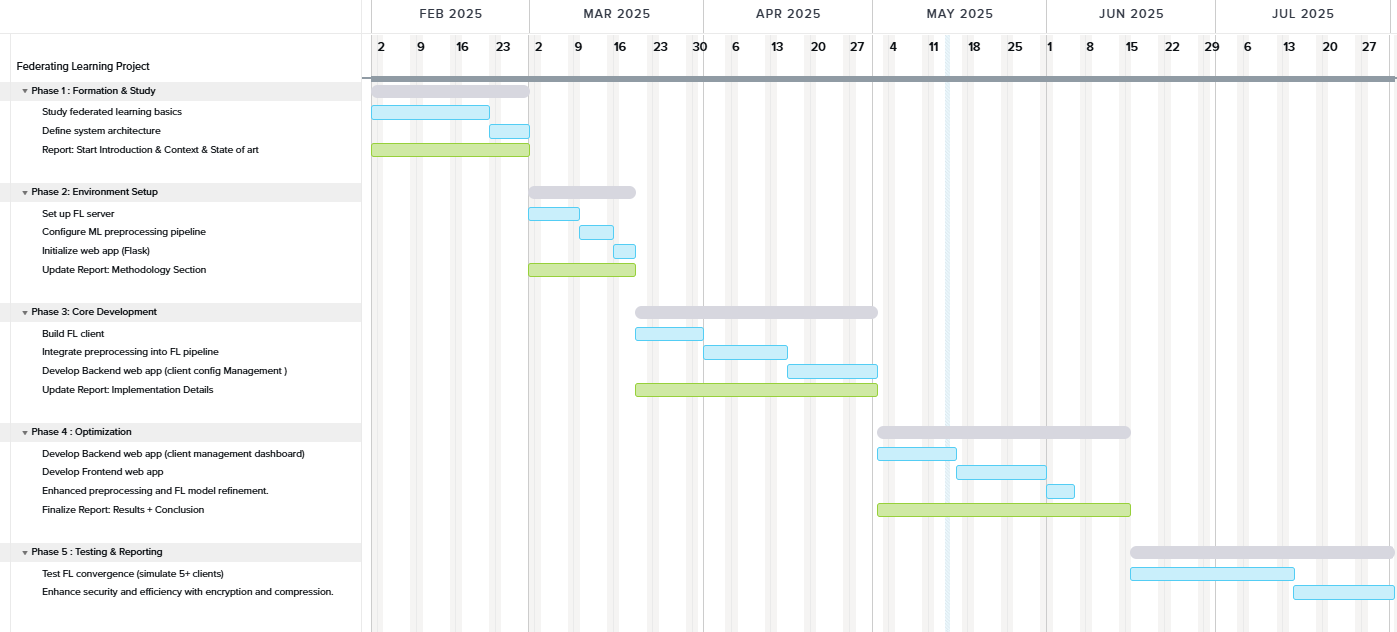
\includegraphics[width=1\linewidth]{Figures/Gantt.png}
    \caption{Gantt Diagram}
    \label{fig:enter-label}
\end{figure}
The Federating Learning Project follows a phased and systematic process to carry out a smooth and effective development. The project is started with Phase 1: Formation and Study, in which it is planned to acquire initial knowledge about federated learning, defining the structure of the system, and establishing the context and state of the art for Report. This phase ensures a clear understanding of the objectives, methodologies, and technological requirements before moving ahead. Following the initial study, Phase 2: Environment Setup is devoted to the installation of the necessary infrastructure. This involves the installation of the federated learning server, machine learning preprocessing pipeline configuration, and web application initialization with Flask. The Report methodology section is also updated to include these advances, with proper documentation of the installation phase.

Once the environment is set up, the project proceeds to Phase 3: Core Development, where the core components of the system are built. This phase includes building the FL client, implementing preprocessing in the federated learning pipeline, and building the backend web app for client configuration management. During this phase, the implementation details of the Report are also updated to track progress.

The Optimization Phase (Phase 4) is used to enhance and refine the system.

The backend web application is enhanced to include a client management dashboard, a frontend web application is developed, and additional enhancements are made to the preprocessing and federated learning model. The system is fully functional, efficient, and user-friendly in this phase. Besides, the Results and Conclusion of the Report is finalized, such as knowledge and experience gained in the development and optimization process. Phase 5: Testing and Reporting, the final phase, is crucial in confirming the functionality and security of the system. Convergence of federated learning is tested through simulations involving at least five clients to examine its performance. Additionally, security patches by way of encryption and compression techniques are incorporated to determine data confidentiality and integrity. Every step of the project is carefully planned and executed sequentially with dependencies between tasks to produce a logical progression. This methodical approach guarantees effective and well-documented development, leading to the successful deployment of a federated learning system.

\newpage

\section*{Conclusion}
